\chapter{Soluția propusă}

\section{Arhitectura generală a sistemului}
Platforma este construită pe o arhitectură de tip client-server, în care interfața de utilizator și logica serverului sunt separate și comunică exclusiv prin intermediul unui REST API, fiecare componentă putând fi dezvoltată și întreținută independent de cealaltă. \Cref{fig:system-architecture} prezintă o vedere de ansamblu a sistemului, arătând componentele principale și relațiile dintre ele.

\begin{figure}[htbp]
    \centering
    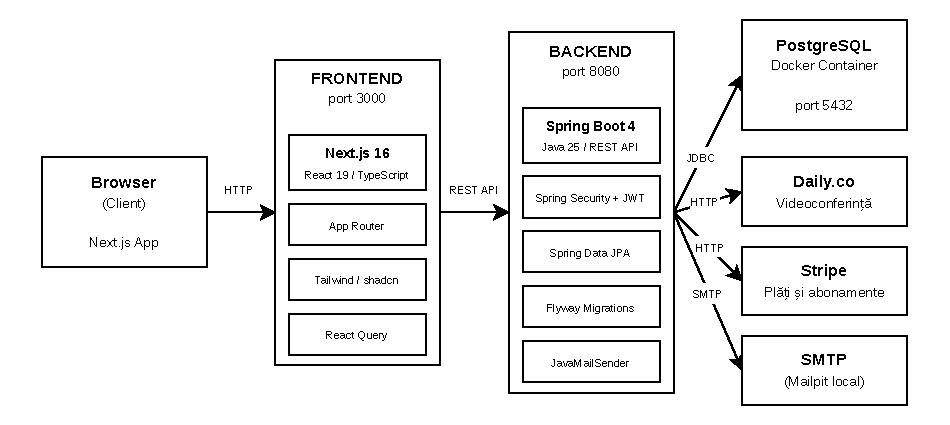
\includegraphics[width=0.8\textwidth]{pics/diagrams/system-architecture.pdf}
    \caption{Arhitectura generală a sistemului}
    \label{fig:system-architecture}
\end{figure}

Componenta client este o aplicație Next.js care rulează în browserul utilizatorului, trimițând cereri HTTP către server și afișând datele primite ca răspuns, fără a deține logica din spatele aplicației sau acces direct la baza de date. Componenta server este o aplicație Spring Boot care expune un REST API, ce procesează cererile primite de la client, aplică regulile aplicației și interacționează cu baza de date și cu serviciile externe, returnând răspunsuri în format JSON. Practic, clientul nu știe cum funcționează serverul și invers, cei doi comunicând doar prin cereri și răspunsuri HTTP bine definite.

Autentificarea se realizează prin token-uri JWT, clientul primind un token la autentificare și incluzându-l în headerul fiecărei cereri ulterioare \cite{jwt}. Serverul verifică validitatea acestuia și extrage identitatea și rolul utilizatorului înainte de a procesa cererea, returnând un răspuns cu codul 401 dacă token-ul lipsește sau nu este valid. Abordarea aceasta face serverul stateless, nefiind nevoie să stocheze sesiuni active ale utilizatorilor.

Baza de date PostgreSQL rulează într-un container Docker separat, serverul conectându-se la aceasta prin JDBC, iar schema bazei de date este gestionată și versionată prin Flyway, care aplică automat migrările SQL la pornirea aplicației.

Serviciile externe, Daily.co pentru sesiunile video, Stripe pentru plăți și abonamente și serverul SMTP pentru emailuri, sunt accesate exclusiv de server prin cereri HTTP, clientul neavând niciun contact direct cu acestea.

\section{Modelul bazei de date}
Baza de date este organizată în mai multe grupuri de tabele, fiecare acoperind un domeniu funcțional distinct al sistemului, toate conectate prin foreign keys care asigură integritatea datelor. Diagrama entitate-relație completă a bazei de date este prezentată în Anexa B (\Cref{fig:er-diagram}).

Primul grup acoperă gestionarea utilizatorilor, tabela \texttt{users} stocând informațiile de bază ale fiecărui utilizator, inclusiv rolul în sistem și statusul contului, ambele câmpuri fiind verificate de server la fiecare cerere autentificată. Al doilea grup acoperă conținutul didactic, cursurile, lecțiile, exercițiile și quiz-urile, formând o ierarhie clară în care fiecare entitate are câmpuri dedicate pentru statusul de publicare și, în cazul cursurilor, pentru statusul de revizuire, controlând ce este vizibil studenților și ce se află în așteptarea aprobării.

Progresul studenților este urmărit prin tabele separate, una pentru progresul la nivel de lecție și alta pentru sesiunile de quiz. Tabela \texttt{quiz\_attempts} stochează răspunsurile date la fiecare întrebare împreună cu momentul de start al sesiunii, permițând serverului să verifice dacă limita de timp a fost respectată la momentul trimiterii.

Sesiunile video sunt reprezentate prin tabela \texttt{meetings}, fiecare sesiune având asociat un profesor, un interval orar planificat și un identificator al camerei din Daily.co, participanții și statusul lor individual (rezervat, prezent sau absent), fiind stocate într-o tabelă separată. Disponibilitatea profesorilor este configurată prin intervale orare recurente săptămânale, pe baza cărora serverul calculează automat sloturile disponibile ținând cont de sesiunile deja rezervate.

Sistemul de facturare folosește mai multe tabele interconectate, abonamentele stocând informațiile despre planul activ al fiecărui student și datele de reînnoire primite de la Stripe, balanța de credite fiind gestionată separat printr-un mecanism care previne deducerea incorectă a creditelor în cazul rezervărilor simultane. Un jurnal de tranzacții înregistrează fiecare modificare a balanței cu motivul aferent, oferind o imagine completă a istoricului de credite.

\section{Componenta client}
Componenta client este dezvoltată în Next.js, folosind App Router, sistemul de rutare bazat pe structura directorului \texttt{app}, în care fiecare director corespunde unei rute sau unui grup de rute cu comportament comun (\Cref{fig:client-structure}).

Structura paginilor este organizată pe niveluri de acces: paginile publice accesibile fără autentificare, paginile disponibile oricărui utilizator autentificat și paginile specifice fiecărui rol. Accesul este verificat la nivelul fiecărei componente, utilizatorul neautorizat fiind redirecționat automat. Paginile specifice profesorului acoperă crearea și gestionarea cursurilor și configurarea disponibilității, în timp ce paginile administratorului acoperă gestionarea utilizatorilor, aprobarea profesorilor și revizuirea cursurilor.

Comunicarea cu serverul este gestionată prin TanStack Query, cunoscut anterior ca React Query, care se ocupă automat de cache-ul datelor, invalidând cache-ul la operații de scriere și reîncărcând informațiile afectate fără a fi nevoie de cod suplimentar \cite{reactquery}. De exemplu, după rezervarea unei sesiuni, lista sesiunilor și balanța de credite se actualizează automat în interfață.

Starea de autentificare a utilizatorului este menținută pe tot parcursul sesiunii și sincronizată între tab-uri. Un utilizator care se deconectează dintr-un tab poate vedea modificarea reflectată automat în toate celelalte tab-uri deschise, fără a fi necesar ca acesta să reîncarce pagina sau să facă altă acțiune.

Pentru interfața vizuală s-au folosit Tailwind CSS și componente din shadcn/ui, primul oferind un sistem de clase care permite stilizarea directă în markup, iar al doilea furnizând componente accesibile și ușor de personalizat care asigură o experiență vizuală consistentă pe întreaga platformă \cite{tailwind}\cite{shadcn}. Aplicația funcționează corect pe orice dimensiune de ecran, layout-ul adaptându-se automat atât pentru desktop, cât și pentru dispozitive mobile, fără a fi nevoie de o versiune separată pentru fiecare.

\begin{figure}[htbp]
    \centering
    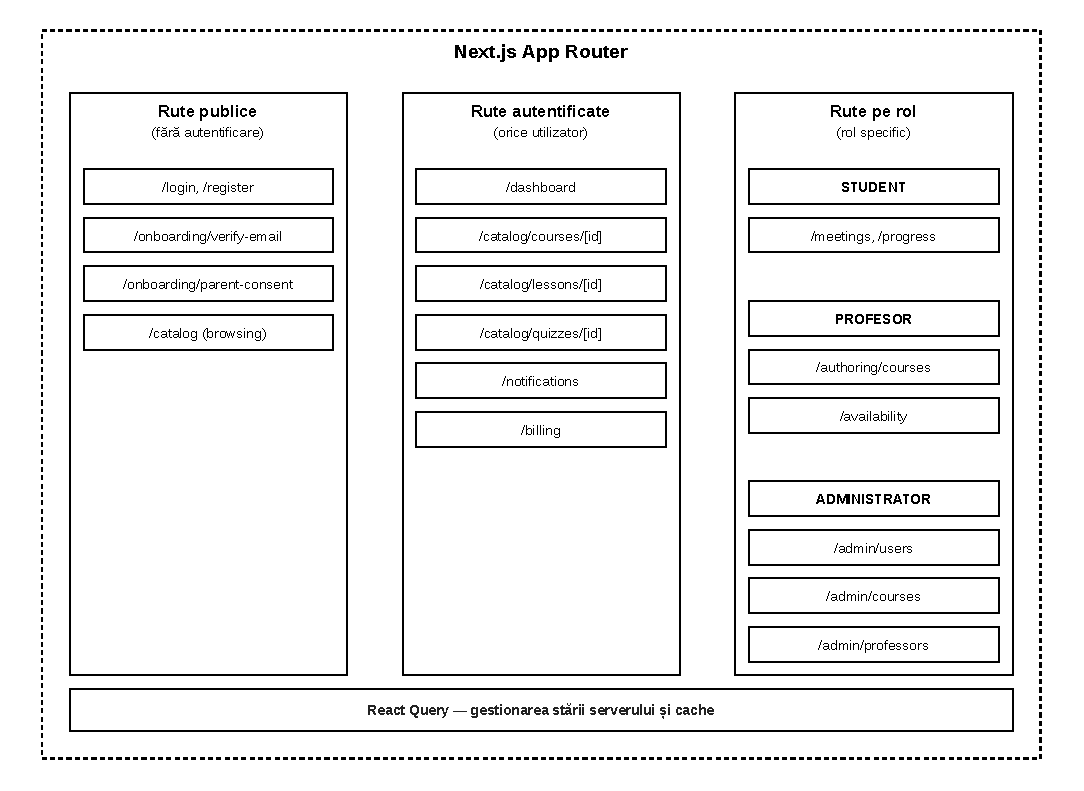
\includegraphics[width=0.8\textwidth]{pics/diagrams/client-structure.pdf}
    \caption{Structura componentei client}
    \label{fig:client-structure}
\end{figure}

\section{Componenta server}
Componenta server este organizată în trei straturi principale cu responsabilități clare, comunicând între ele într-o singură direcție, de la controller spre repository. \Cref{fig:server-layers} prezintă această structură.

Stratul „controller” gestionează cererile HTTP primite de la client, fiecare controller acoperind un domeniu funcțional specific, autorizarea realizându-se prin adnotarea \texttt{@PreAuthorize} care verifică rolul utilizatorului înainte de a permite accesul la o metodă. Validarea datelor trimise de client se face tot la acest nivel, serverul returnând automat un răspuns cu codul 400 și detaliile erorii dacă datele nu respectă constrângerile definite.

Stratul „service” conține logica aplicației și coordonează operațiile între mai multe repository-uri atunci când este necesar. La rezervarea unei sesiuni, de exemplu, serviciul verifică disponibilitatea profesorului, numărul creditelor studentului și absența conflictelor, toate acestea înainte de a crea o intrare în baza de date și a deduce creditele. Tranzacțiile bazei de date sunt gestionate la acest nivel, operațiile care implică mai multe modificări grupându-se într-o singură tranzacție pentru a asigura că fie toate reușesc, fie niciuna nu este aplicată.

Stratul „repository” asigură accesul la baza de date prin Spring Data JPA, expunând operații standard și metode personalizate generate automat pe baza numelui metodei sau definite explicit prin adnotarea \texttt{@Query} pentru interogări mai complexe.

Securitatea serverului este asigurată prin Spring Security, configurat să intercepteze toate cererile primite, să extragă și să valideze token-ul JWT din header și să populeze contextul de securitate cu identitatea utilizatorului, permițând astfel ca adnotările \texttt{@PreAuthorize} să funcționeze corect.

\begin{figure}[htbp]
    \centering
    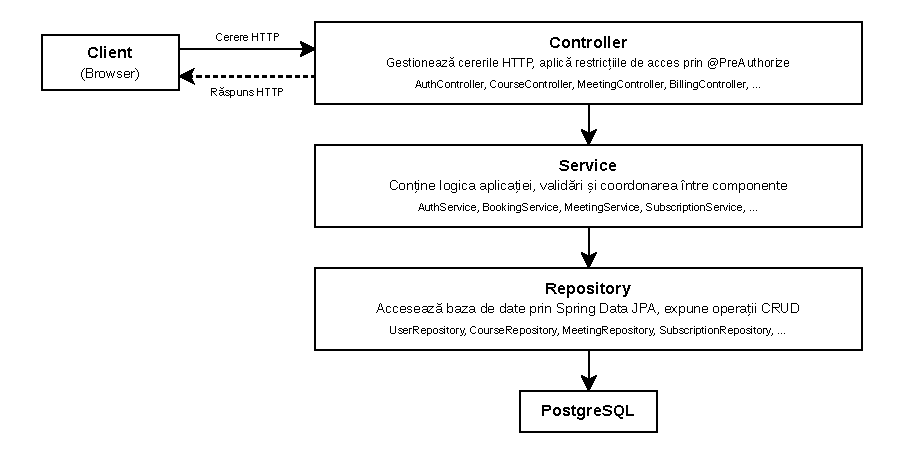
\includegraphics[width=0.8\textwidth]{pics/diagrams/server-layers.pdf}
    \caption{Structura componentei server}
    \label{fig:server-layers}
\end{figure}

\section{Integrări externe}
Platforma integrează trei servicii externe pentru funcționalități specializate care ar fi necesitat un efort semnificativ de implementare de la zero.

Integrarea cu Daily.co gestionează ciclul de viața al camerelor de sesiune video. Serverul creează programatic o cameră la momentul rezervării și furnizează clientului token-ul de acces necesar pentru a intra în cameră direct din interfața platformei, fără a fi redirecționat în altă aplicație. Tot ce știe clientul despre sesiunea video este un URL și un token, restul comunicării cu Daily.co realizându-se exclusiv pe server. La anularea sau finalizarea unei sesiuni, camera este ștearsă automat pentru a nu acumula resurse neutilizate.

Integrarea cu Stripe acoperă întregul flux de facturare, de la crearea unui abonament și procesarea primei plăți până la reînnoirile recurente și anulările. Serverul primește notificări despre evenimentele de plată prin webhook-uri și actualizează statusul abonamentului și balanța de credite a studentului în consecință, idempotența procesării fiind asigurată prin stocarea identificatorului fiecărui eveniment procesat pentru a evita procesarea duplicatelor. Studentul poate gestiona singur abonamentul printr-un portal Stripe accesat direct din platformă.

Integrarea cu serverul SMTP este folosită pentru trimiterea emailurilor de verificare la înregistrare, a solicitărilor de consimțământ parental pentru utilizatorii minori și a notificărilor despre deciziile administratorului, emailurile fiind trimise asincron pentru a nu bloca procesarea celorlalte cereri.
